\begin{tikzpicture}[
  FORK/.style={circle , draw=none , fill=white , inner sep=0 },
  lbl1/.style={circle , draw=none , fill=white , inner sep=0 
              , font=\tiny},
  lbl2/.style={circle , draw=none , fill=white , inner sep=0 
              , font=\tiny},
  symbol/.style={circle , draw=none , fill=yellow , inner sep=0 },
  lit/.style={circle , draw=none , fill=green , inner sep=0 }
]
\tikzset{edge from parent/.style=
  {draw,
  edge from parent path={(\tikzparentnode.south)
  -- +(0,-8pt)
  -- (\tikzchildnode)}}}
  
\tikzset{level 0+/.style={level distance=1.3cm}}
  
\Tree [ \edge node [pos=0 , FORK] {$\equiv$};
        [ \edge node [pos=0 , FORK] {$+$};
          [ [ \edge[dashed] node [pos=0.3 , symbol] {0}; $r_1$ ]
            [ \edge[dashed] node [pos=0.3 , symbol] {2}; $l_1$ ]
          ]
          \edge node [pos=0 , FORK] {$+$};
          [ [ \edge node [pos=0.3 , lit] {0}; $r_1\vdash r_2$ ]
            [ \edge[dashed] node [pos=0.3 , symbol] {1}; $r_1\vdash k_1$ ]
            [ \edge node [pos=0 , FORK] {$+$};
               [ \edge[dashed] node [pos=0.3 , symbol] {1}; $l_1\vdash l_2$ ]
              \edge node [pos=0 , FORK] {$+$};
               [ \edge[dashed] node [pos=0.3 , symbol] {0}; $l_2\vdash l_3$  ]
            ]
          ]
        ]
        \edge node [pos=0 , FORK] {$\equiv$};
        [ [ \edge[dashed] node[pos=0.3 , symbol] {0}; $r_2\vdash RI$ ] 
          [ \edge node [pos=0 , FORK] {$+$};
            [ [ \edge[dashed] node[pos=0.3 , symbol] {1}; $k_1\vdash k_2$ ]
              [ \edge node [pos=0 , FORK] {$+$};
                [ \edge[dashed] node [pos=0.3 , symbol] {2}; $l_3\vdash l_4$ ]
                \edge node [pos=0 , FORK] {$+$};
                [ \edge[dashed] node [pos=0.3 , symbol] {1}; $l_4\vdash ASSOC$ ]
              ]
            ]
            \edge node [pos=0 , FORK] {$+$};
            [ \edge[dashed] node [pos=0.3 , symbol] {0}; $k_2\vdash COMM$ ]
          ] 
        ] 
      ];
\end{tikzpicture}
